\documentclass[a4paper,10pt,fleqn]{article}

\usepackage{../layout/layout}

\title{Produktbeschreibung Funktion}
\author{Yannik Küng}

\begin{document}

\maketitle
\clearpage
\tableofcontents
\clearpage

Aufgrund der Resultate der Evaluation der Lösungsprinzipien wurde beschlossen 
das Konzept der stationären Abschussvorrichtung (Drehturm) weiter 
auszuarbeiten. 
%
Hierbei handelt es sich um ein nicht fahrbares, autonom arbeitendes Gerät mit 
einer in radialer Richtung drehbarer Abschussvorrichtung. Der gesamte Aufbau 
des Abschussmechanismus inklusive Balllager befindet sich auf einer drehbaren 
Plattform, welche auf einem geeigneten Ständer platziert ist. Die Plattform 
wird durch einen Schrittmotor und einer Zahnradübersetzung präzise in Position 
gebracht. Der Abschusswinkel in horizontaler Richtung ist hierbei fixiert. 
%
Die Abschussvorrichtung besteht im Wesentlichen aus einem Balllager, einer 
Ballnachführung und einem sich schnell drehenden Rad, welches die Bälle auf 
die gewünschte Abschussgeschwindigkeit beschleunigt. Die Bauweise dieser drei 
Komponenten soll integral erfolgen, wobei das längliche, Quaderförmige 
Balllager als Hauptstruktur dient. Auf diesem sind sowohl das Rad für die 
Ballbeschleunigung sowie die Komponenten der Ballnachfürung befestigt.
%
Das Rad für die Ballbeschleunigung soll auf der Oberseite des Balllagers 
positioniert sein. Auf der Unterseite wird eine geeignete Platte befestigt um 
so den benötigten Anpressdruck zu erzeugen. 
%
Die Ballnachführung wird durch ein im inneren des Balllager verlaufendes Band 
realisiert. Dieses wird durch eine an der Aussenseite des Balllagers 
angebrachten Trommel aufgewickelt und zieht so die einzelnen Bälle Richtung 
Abschussrad.
%
Der Korb wird mittels einer Bilderkennungssoftware, die auf einem 
angeschlossenen PC betrieben wird, erkannt und die so gewonnenen 
Positionsdaten an die entsprechenden Ansteuerungskomponenten gesendet. Diese 
können anschliessend den Winkel in horizontaler Richtung, sowie die 
Abschussgeschwindigkeit und somit die Schussweite, mit der Drehzahl des 
Beschleunigungsrades regeln.
%
Die Übertragung des Startsignals, sowie die Anzeige des Endsignals erfolgt per 
Wlan über einen zweiten Laptop.

\section{List some items}
\begin{itemize}
    \item First item
    \item Second item
    \item Another item
    \begin{itemize}
        \item Subitem
        \begin{itemize}
            \item Subsubitem
            \begin{itemize}
                \item Subsubsubitem --- Just joking, You should not use such 
                    deep nested Lists.
            \end{itemize}
        \end{itemize}
    \end{itemize}
    \item[+] Even special symbols are possible
    \item[$\sum$] Which can also be in math mode
\end{itemize}

\subsection{Enumered list}
\begin{enumerate}
    \item First item
    \item Second item
    \item Another item
    \begin{enumerate}
        \item Subitem
        \begin{enumerate}
            \item Subsubitem
            \begin{enumerate}
                \item Subsubsubitem --- Just joking, You should not use such 
                    deep nested Lists.

            \end{enumerate}
        \end{enumerate}
    \end{enumerate}
\end{enumerate}

\clearpage
\section{Enumered list}
\begin{enumerate}
    \item First item
    \item Second item
    \item Another item
    \begin{enumerate}
        \item Subitem
        \begin{enumerate}
            \item Subsubitem
            \begin{enumerate}
                \item Subsubsubitem --- Just joking, You should not use such 
                    deep nested Lists.

            \end{enumerate}
        \end{enumerate}
    \end{enumerate}
\end{enumerate}

\subsection{Code}
\lstsettinglatex
\lstinputlisting{list_enum.tex}

\clearpage
\section{Table with "'Zebra pattern"'}
\begin{table}[h!]
    \begin{zebralongtable}{@{}ll}
        \rowcolor{gray} 
        Component   & Value \\
        R102        & 10k$\Omega$ \\
        R103        & 12k$\Omega$ \\
        C105        & 10nF \\
        U1          & NE555 \\
    \end{zebralongtable}
    \caption{Example of a BOM}
    \label{tab_bom}
\end{table}

\clearpage
\section{Image}

\begin{figure}[h!]
    \centering
    \includegraphics[width=0.3\textwidth]{fig/example.pdf}
    \caption{Example image}
    \label{fig:example}
\end{figure}
Above you see an example picture in Abbildung \ref{fig:example}. 

\subsection{Code}
\lstsettinglatex
\lstinputlisting{image.tex}

\clearpage
\section{Formulas}
There are two ways to typeset math. 

\subsection{Inline}
Formulas can be entered inside the text. Therefore the formulas need to be 
between \verb!$!. \\
Example: 
Einstein said that $E = m \cdot c^2$. 

\subsection{Separate paragraph}
Formulas can be defined in a separate paragraph. Formulas typeset this way 
start with \verb!\[! and end with \verb!\]!. \\
Example: 
Einsteinsaid that
\[ E = m \cdot c^2 \]

\subsection{Code}
\lstsettinglatex
\lstinputlisting{math.tex}

\clearpage
\section{Often used mathematical symbols}

\subsection{Basic Symbols}
\[ + ~ - ~ \cdot ~ / ~ \div \]
\[ \to ~ \infty \]
\[ \alpha ~ \beta ~ \gamma ~ \delta ~ \varphi \]
\[ \vartheta ~ \pi ~ \kappa ~ \tau ~ \omega \]
\[ \Gamma ~ \Delta ~ \Phi ~ \Lambda ~ \Omega \]

\subsection{Basic constructs}
\[ a_{b} \qquad a^{b} \qquad {a_{b}}^{c} \]
\[ \frac{a}{b} \qquad \left( \frac{a}{b} \right) \]
\[ \sqrt{a} \qquad \sqrt[5]{a} \]
\[ \lim\limits_{a \to \infty} c \]
\[ \sum\limits_{a}^{b}c \qquad \int\limits_{a}^{b}c \]

\subsection{Code}
\lstsettinglatex
\lstinputlisting{math-use.tex}

\clearpage
\section{Listing with C sytax highlighting}
\lstsettingc
\begin{lstlisting}
#include <stdio.h>

/**
 * main function
 * Prints a "Hello World"
 */
int main(int argc, char **argv)
{
    printf("Hello world\n");    // Prints some text
    return 0;
}
\end{lstlisting}

\clearpage
\section{Listing from an external file}

\subsection{Code}
\lstsettinglatex                    % Setting up for LaTeX highlighting
\lstinputlisting{listing_ext.tex}   % Include external file listing_ext.tex

\end{document}
